\def\year{2019}\relax
%File: formatting-instruction.tex
\documentclass[letterpaper]{article} %DO NOT CHANGE THIS
\usepackage{aaai19}  %Required
\usepackage{times}  %Required
\usepackage{helvet}  %Required
\usepackage{courier}  %Required
\usepackage{url}  %Required
\usepackage{graphicx}  %Required
% insert here the call for the packages your document requires
\usepackage{xspace}
\usepackage{times}
\usepackage{amsmath,amssymb,amsfonts}
\usepackage{verbatim}
\usepackage{subfigure}
\usepackage{multirow}
\usepackage{psfrag,graphicx,epsfig,epsf}
\usepackage{graphics}
\usepackage{latexsym}
\usepackage[ruled,linesnumbered, noend]{algorithm2e}
\usepackage{fancyhdr}
\usepackage{fullpage}
\usepackage{wrapfig}
\usepackage{subfigure}
\usepackage{setspace}
%\usepackage[bookmarks=true]{hyperref}
%\usepackage{multicol}
\usepackage{color}

\frenchspacing  %Required
\setlength{\pdfpagewidth}{8.5in}  %Required
\setlength{\pdfpageheight}{11in}  %Required
%PDF Info Is Required:
  \pdfinfo{
/Title (Integrated Task and Motion Planning for Manipulation)
/Author (Rahul Shome)}
\setcounter{secnumdepth}{0}

  
\begin{document}

\title{Integrated Task and Motion Planning for Dexterous Prehensile Manipulation}
\author{Rahul Shome}
\maketitle

\newcommand{\danh}[2][1=]{\todo[linecolor=blue,
			backgroundcolor=blue!5,bordercolor=black,#1]{DH:#2}}
\newcommand{\kb}[2][1=]{\todo[linecolor=green,
			backgroundcolor=green!5,bordercolor=black,#1]{KB:#2}}
\newcommand{\ks}[2][1=]{\todo[linecolor=red,
			backgroundcolor=red!5,bordercolor=black,#1]{KS:#2}}
\newcommand{\rs}[2][1=]{\todo[linecolor=orange,
			backgroundcolor=orange!10,bordercolor=black,#1]{RS:#2}}
\newcommand{\jy}[2][1=]{\todo[linecolor=black,
			backgroundcolor=black!5,bordercolor=black,#1]{JJ:#2}}

%%% Mathematical Definitions
\newcommand{\reals}{\mathbb{R}}
\newcommand{\integers}{\mathbb{Z}}

%%% Definitions for Workspace, Objects, Manipulator
\newcommand{\Wspace}{\mathcal{W}}
\newcommand{\Objects}{\mathcal{O}}
\newcommand{\Manip}{\mathcal{M}}
\newcommand{\nobj}{k}

%% Definitions for Object stuff
\newcommand{\Pspace}{\mathcal{P}}
\newcommand{\Pstable}{\mathcal{P}^s}
\newcommand{\pose}{p}
\newcommand{\GeomObj}{\mathcal{WO}}
\newcommand{\Arrange}{\mathcal{A}}
\newcommand{\Pumped}{\mathcal{A^P}}
\newcommand{\pumpedarr}{\alpha^{\mathcal{P}}}

%% Definitions for Manipulator stuff
\newcommand{\Qspace}{\mathcal{Q}}
\newcommand{\GeomManip}{\mathcal{WM}}

%% Definitions for problem and state space
\newcommand{\Tspace}{\mathbb{T}} 
\newcommand{\Xspace}{\mathbb{X}}
\newcommand{\paths}{\Pi}

%% Manipulation roadmap definition
\newcommand{\roadmap}{\mathcal{R}}
\newcommand{\graph}{\mathcal{G}}
\newcommand{\nodes}{\mathcal{V}}
\newcommand{\node}{{v}}
\newcommand{\edges}{\mathcal{E}}
\newcommand{\edge}{{e}}
\newcommand{\prmstar}{{\tt PRM$^*$}}

\newcommand{\rpg}{${\tt RPG}$}

\newcommand{\local}{\mathcal{L}}

\newcommand{\prm}{{\tt PRM}}
\newcommand{\kprmstar}{{\tt k-PRM$^*$}}
\newcommand{\rrt}{{\tt RRT}}
\newcommand{\rrtdrain}{{\tt RRT-Drain}}
\newcommand{\rrg}{{\tt RRG}}
\newcommand{\est}{{\tt EST}}
\newcommand{\rrtstar}{{\tt RRT$^*$}}
\newcommand{\srrt}{{\tt RDG}}
\newcommand{\bvp}{{\tt BVP}}
\newcommand{\rdg}{{\tt RDG}}
\newcommand{\lrg}{{\tt LRG}}
\newcommand{\alg}{{\tt ALG}}
\newcommand{\upump}{{\tt UPUMP}}
\newcommand{\prxpump}{{\tt RPG}}
\newcommand{\fixed}{{\tt Fixed}-$\alpha$-\rdg}
\newcommand{\nrob}{k}
\newcommand{\cons}{K}

\newcommand{\frnodes}{V_f}
\newcommand{\frnode}{v_f}
\newcommand{\grnodes}{V_g}
\newcommand{\grnode}{v_g}
\newcommand{\fredges}{E_f}
\newcommand{\fredge}{e_f}
\newcommand{\gredges}{E_g}
\newcommand{\gredge}{e_g}
\newcommand{\kedges}{E_{\cons}}
\newcommand{\kedge}{e_{\cons}}
\newcommand{\safe}{q_s^{\mathcal{M}}}
\newcommand{\hedges}{E_H}
\newcommand{\hedge}{e_H}
\newcommand{\hnodes}{V_H}
\newcommand{\hnode}{v_H}
\newcommand{\hgraph}{H}
\newcommand{\nblank}{b}
\newcommand{\config}{C}
\newcommand{\cquery}{\mathbb{C}}
\newcommand{\pumped}{P}
\newcommand{\pumpedgraph}{\mathcal{G}_P}
\newcommand{\pnodes}{V_P}
\newcommand{\pnode}{v_P}
\newcommand{\pedges}{E_P}
\newcommand{\pedge}{e_P}
\newcommand{\signs}{\Sigma}
\newcommand{\sign}{\sigma}
\newcommand{\gsign}{\sigma_{\pumpedgraph}}
\newcommand{\cedges}{E_c}
\newcommand{\constraints}{\tt c}


\newenvironment{myitem}{\begin{list}{$\bullet$}
{\setlength{\itemsep}{-0pt}
\setlength{\topsep}{0pt}
\setlength{\labelwidth}{0pt}
%\setlength{\labelsep}{0pt}
\setlength{\leftmargin}{10pt}
\setlength{\parsep}{-0pt}
\setlength{\itemsep}{0pt}
\setlength{\partopsep}{0pt}}}%
{\end{list}}

%\newtheorem{theorem}{Theorem}
%\newtheorem{definition}[theorem]{Definition}
%\newtheorem{proposition}[theorem]{Proposition}
%\newtheorem{corollary}[theorem]{Corollary}
%\newtheorem{axiom}[theorem]{Axiom}
%\newtheorem{lemma}[theorem]{Lemma}
%\newtheorem{problem}{Problem}
%\newtheorem{prob}[theorem]{Problem}
%\newtheorem{conjecture}[theorem]{Conjecture}
%\newtheorem{obj}[theorem]{Objective}
%\newtheorem{prop}[theorem]{Property}
%\newtheorem{schedule}[theorem]{Schedule}


%\newtheorem{definition}{\bf Definition}
%\newtheorem{assumption}{\bf Assumption}
%\newtheorem{thm}{\bf Theorem}
%\newtheorem{requirement}{\bf Requirement}
%\newtheorem{lemmma}{\bf Lemma}
%\newtheorem{coro}{\bf Corollary}





%%%%%%%%%%%%%%%%%%%%%%%%%%%%%%%%%%%%
%% Nick Saving space
%%%%%%%%%%%%%%%%%%%%%%%%%%%%%%%%%%%%
% Space between figure and caption
%\setlength{\abovecaptionskip}{-2.5pt}
%\setlength{\belowcaptionskip}{-6pt}
%% Space between text and figs
%\setlength{\dbltextfloatsep}{2pt plus 1.0pt minus 1.0pt}
%\setlength{\textfloatsep}{2pt plus 1.0pt minus 1.0pt}
%\setlength{\intextsep}{2pt plus 1.0pt minus 1.0pt}
%% Space between equations and text
%\setlength{\belowdisplayskip}{0pt} \setlength{\belowdisplayshortskip}{2pt}
%\setlength{\abovedisplayskip}{0pt} \setlength{\abovedisplayshortskip}{2pt}

\newcommand{\dof}{{\tt DoF}}

\newcommand{\mam}{$\mathcal{G}_{\tt MAM}$}
\newcommand{\pr}{\ensuremath{\mathbb{P}}}


\newcommand{\rad}{\ensuremath{r(n)}}
\newcommand{\radstar}{\ensuremath{r^*(n)}}
\newcommand{\radi}{\ensuremath{r_i(n)}}
\newcommand{\radj}{\ensuremath{r_j(n)}}
\newcommand{\crossrad}{\ensuremath{r_R(n)}}
\newcommand{\crossradstar}{\ensuremath{r^*_R(n)}}
\newcommand{\impcrossrad}{\ensuremath{\hat r_R(n)}}
\newcommand{\allimpcrossrad}{\ensuremath{\hat r_{R}(n^R)}}
\newcommand{\ki}{\ensuremath{k_i(n)}}
\newcommand{\kj}{\ensuremath{k_j(n)}}

%% Manipulation roadmap definition
\newcommand{\mmgraph}{\ensuremath{\mathbb{G}}}
\newcommand{\mmgimp}{\hat\mmgraph}
\newcommand{\mmgexp}{\mmgraph}
\newcommand{\aograph}{\ensuremath{\mathbb{G}^{AO}}}
\newcommand{\tree}{\ensuremath{\mathbb{T} \ }}
\newcommand{\mmnodes}{\mathbb{\hat V}}
\newcommand{\mmedges}{\mathbb{\hat E}}
\newcommand{\mmnodestpprm}{\mathbb{V}_{\chi_i}}
\newcommand{\mmedgestpprm}{\mathbb{E}_{\chi_i}}
\newcommand{\mmnode}{\mathbb{\hat v}}
\newcommand{\mmedge}{\mathbb{\hat e}}
\newcommand{\sprmstar}{Soft-\ensuremath{ {\tt PRM} }}
\newcommand{\irs}{\ensuremath{ {\tt IRS} }}
\newcommand{\spars}{{\tt SPARS}}
\newcommand{\drrt}{\ensuremath{{\tt dRRT}}}
\newcommand{\drrtstar}{\ensuremath{{\tt dRRT^*}}}
\newcommand{\dadrrtstar}{\ensuremath{\tt da\_dRRT^*}}

\newcommand{\sig}{{\tt SIG}}
\newcommand{\rmaps}{\ensuremath{\mathfrak{R}}}

\newcommand{\mmprm}{\ensuremath{\text{Random-}{\tt MMP}}}
\newcommand{\astar}{{\ensuremath{\tt A^{\text *}}}}
\newcommand{\mstar}{{\tt M^{\text *}}}
\newcommand{\opens}{P_{Heap}}


\newcommand{\cost}{\textup{cost}}



%\newcommand*{\qed}{\hfill\ensuremath{\square}}

\newcommand{\kiril}[1]{{\color{blue} \textbf{Kiril:} #1}}
\newcommand{\chups}[1]{{\color{green} \textbf{Chuples:} #1}}
\newcommand{\rahul}[1]{{\color{red} \textbf{Rahul:} #1}}

\newcommand{\T}{\mathcal{T}}

% Dual Arm
\newcommand{\leftrm}{\ensuremath{\mathbb{R}_{l}}  }
\newcommand{\rightrm}{\ensuremath{\mathbb{R}_{r}}  }
\newcommand{\leftmetric}{\ensuremath{\mathbb{P}_{l}}  }
\newcommand{\rightmetric}{\ensuremath{\mathbb{P}_{r}}  }
\newcommand{\cfull}{\ensuremath{\mathbb{C}_{{\rm full}}}  }
\newcommand{\cfree}{\ensuremath{\mathbb{C}_{{\rm free}}}  }
\newcommand{\cobs}{\ensuremath{\mathbb{C}_{{\rm obs}}}  }
\newcommand{\cleft}{\ensuremath{\mathbb{C}_{{l}}}  }
\newcommand{\cright}{\ensuremath{\mathbb{C}_{{r}}}  }
\newcommand{\cshared}{\ensuremath{\mathbb{C}_{{s}}}  }
\newcommand{\cgoal}{\ensuremath{q_{{\rm goal}}}  }
\newcommand{\cstart}{\ensuremath{q_{{\rm start}}}  }

\newcommand{\gimpleft}{\ensuremath{\hat\mmgraph_l}}
\newcommand{\gimpright}{\ensuremath{\hat\mmgraph_r}}


\newcommand{\xrand}{\ensuremath{x^{\textup{rand} \ }}}
\newcommand{\xnear}{\ensuremath{x^{\textup{near} \ }}}
\newcommand{\xnew}{\ensuremath{x^{\textup{n}} \ }}
\newcommand{\xlast}{\ensuremath{x^{\textup{last} \ }}}
\newcommand{\xparent}{\ensuremath{x^{\textup{best} \ }}}

\newcommand{\lr}{\ensuremath{\mathbb{R}_{ls}}}
\newcommand{\rr}{\ensuremath{\mathbb{R}_{sr}}}
\newcommand{\lp}{\ensuremath{\mathbb{P}_{l}}}
\newcommand{\rp}{\ensuremath{\mathbb{P}_{r}}}

\newcommand{\motoman}{{\tt Motoman}}
\newcommand{\baxter}{{\tt Baxter}}
\newcommand{\ao}{{\tt AO}}

\newcommand\inlineeqno{\stepcounter{equation}\ (\theequation)}

\newcommand{\chomp}{\ensuremath{\tt CHOMP } }

\newtheorem{assumption}{Assumption}

\newcommand{\W}{\mathcal W}
\newcommand\perm[2][\^n]{\prescript{#1\mkern-2.5mu}{}P\_{#2}}
\newcommand\comb[2][\^n]{\prescript{#1\mkern-0.5mu}{}C\_{#2}}
\newcommand{\objectset}{\mathcal{O}}
\newcommand{\object}{o}
\newcommand{\workspace}{\mathcal{W}}
\newcommand{\taskspace}{\mathcal{T}}
\newcommand{\arrangement}{A}
\newcommand{\oar}{p}
\newcommand{\manipulators}{\mathcal{M}}
\newcommand{\manipulator}{\mathit{m}}
\newcommand{\arm}{m}
\newcommand{\arms}{\mathcal{M}}
\newcommand{\taskset}{\mathcal{T}}
\newcommand{\task}{\mathit{T}}
\newcommand{\sol}{\Pi}
\newcommand{\state}{q}

\newcommand{\Aspace}{\mathcal{A}}
\newcommand{\Afree}{\mathcal{A}_{\rm val}}
\newcommand{\ainit}{A_{\rm init}}
\newcommand{\atarget}{A_{\rm goal}}
\newcommand{\soma}{{\tt soma}}
\newcommand{\coma}{\ensuremath{{\omega}}}
\newcommand{\scoma}{\ensuremath{{{\Omega}}}}
\newcommand{\qset}{\mathcal{Q}}
\newcommand{\startq}{S}
\newcommand{\targetq}{T}

\newcommand{\act}{a}
\newcommand{\actset}{\mathbb{A}}
\newcommand{\trajset}{{\D}}
\newcommand{\moveset}{\bar{\mathcal{O}}}
\newcommand{\home}{Q}
\newcommand{\scomaset}{\{\scoma\}}
\newcommand{\tour}{{\Gamma}}
\newcommand{\tspgraph}{\graph_{\tour}}
\newcommand{\tspnodes}{\nodes_{\tour}}
\newcommand{\tspedges}{\edges_{\tour}}
\newcommand{\algo}{{\tt{TOM}}\xspace}
\newcommand{\kuka}{{\tt{Kuka }}}
\newcommand{\D}{D}
\newcommand{\sininv}{\sin^{-1}}
\newcommand{\cosinv}{\cos^{-1}}
\newcommand{\milp}{{\tt{MILP}}\xspace}
%%%%%%%%%%%%%%%%%%%%%%%%%%%%%%
%Caption model
\newcounter{model}
%\addtocounter{model}{1}
\newenvironment{model}
{\refstepcounter{model}}
{\begin{center}
\textbf{Model. }~\themodel
\end{center}
\medskip}
%%%%%%%%%%%%%%%%%%%%%%%%%%%%%%
\definecolor{darkgreen}{RGB}{30,150,30}
% \newcommand{\commentdel}[1]{{\color{magenta} #1}}
\newcommand{\commentdel}[1]{{\color{magenta}}}
%\newcommand{\commentadd}[1]{{\color{darkgreen} #1}}
 \newcommand{\commentadd}[1]{{#1}}

\newcommand\blfootnote[1]{%
  \begingroup
  \renewcommand\thefootnote{}\footnote{#1}%
  \addtocounter{footnote}{-1}%
  \endgroup
}


\newcommand{\cspace}{\mathbb{C}}
\newcommand{\carms}{\cspace_{\arms}}
\newcommand{\objectmotion}{\mathbb{A}}

\begin{abstract}
A variety of applications in industrial and service robotics settings require efficient solutions to manipulation tasks. The notion of optimal solutions to these problems must address the nuances of optimal task planning\cite{vega2016asymptotically}. The complexity of the problem in the context of manipulation arises out of multiple typically high-dimensional dexterous arms, a large possible set of grasps, and necessary close contacts. Studying the properties necessary to preserve the asymptotic optimality of the underlying algorithm in the domain of dexterous, prehensile manipulation, the work will also propose efficient algorithms that can yield high-quality solutions quickly.
\end{abstract}

\section{Related Work}
Previous work \cite{vega2016asymptotically} has explored the theoretical conditions necessary for preserving asymptotic optimality for planning in a multi-modal setting. Such a search in this multi-modal space can also be accelerated with the use of angelic heuristics \cite{vega2018admissible} appropriate for the domain and with appropriate abstraction.

The work highlights the need for rigor in consideration of
\begin{enumerate}
\item \textbf{Mode transitions}: In the context of manipulation these refer to prehensile grasps, and contact of the object on resting surfaces.
\item \textbf{Abstractions and Heuristics}: The existence of heuristics in this domain can guide the search between modes as well as within modes.
\end{enumerate}

\section{1-arnm 1 object pick-and-place}
There has been recent work \cite{schmitt2017optimal} proposing an optimal framework, demonstrated by the authors to be fast and efficient at coming up with solutions to prehensile manipulation problems. There has not been additional work to make these results reconcile with the theoretical underpinnings \cite{vega2016asymptotically}.


\section{Multi-arm Planning}
Recent work \cite{Dobson:2017aa,shome2017improving} has provided an efficient asymptotically optimal framework $\mathtt{dRRT}^*$ for multi-robot motion planning problems which provide 
\begin{enumerate}
\item \textbf{Scalability benefits}: Compared to the application of sampling based algorithms like $\mathtt{PRM}^*$ and $\mathtt{RRT}^*$ to these domains, $\mathtt{dRRT}^*$ scales to much larger number of robots and configuration spaces.
\item \textbf{High Quality Heuristics}: Using the estimate of shortest paths that exist on the underlying constituent roadmaps, $\mathtt{dRRT}^*$ can efficiently guide the search to promising high quality solutions quickly.
\item \textbf{High Quality Anytime Behavior}: The algorithm also provides high quality solutions fast and asymptotically improves upon them.
\end{enumerate}



\section{Applications in Manipulation Task Planning}
The manipulation task even in the single arm form poses a variety of modes over which the solution lies, as outlined in previous work \cite{dobson2015planning}. An instance of the modes and mode transitions for 
Prehensile multi-arm manipulation task planning poses a variety of challenges which can be classified based on the increasing level of complexity and the search space. The applications include large scale pick-and-place or sorting tasks, as may arise in warehouse automation, service robotics or waste management. 

\begin{figure}[h]
\centering
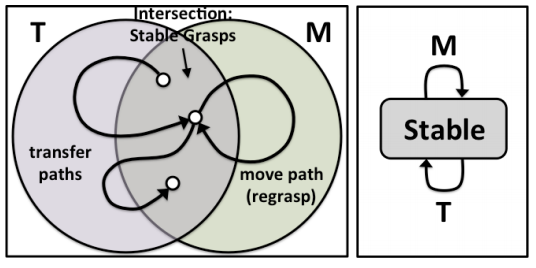
\includegraphics[width=0.42\textwidth]{figures/single_arm}
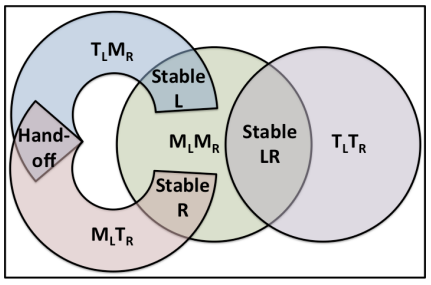
\includegraphics[width=0.42\textwidth]{figures/dual_arm}
\caption{The mode transition diagram for a single arm (\textit{top}), and for two arms (\textit{bottom}), manipulating 1 object. $M$ refers to the moves, and $T$ refers to the transfers of the arms. In the two arm case, the arms are indexed by $L$ and $R$ respectively.
}
\label{fig:single_dual_modes}
\end{figure}

\subsection{2-arm, 1 object pick-and-place}
This is the simplest instance of a multi-arm task planning problem which involves the coordination of 2 arms in a shared workspace to execute an arbitrary pick-and-place of an object that is graspable by at least one arm in its starting pose, and at least one arm in its target pose. Only one arm at a time is sufficient to grasp and move the object.

The sort of modes this introduces include:
\begin{enumerate}
\item \textbf{Moves}: The arms moving without the object grasped. This only involves coordination of the arms to avoid obstacles, the object and each other. In such a mode, the object is resting in a stable fashion on a support surface.
\item \textbf{Transfers}: Either arm can grasp the object, in any valid relative configuration that enforces a stable, prehensile grasp. Any motion of the arm induces a motion of the object while preserving the relative configuration of the object and the end-effector. 
\end{enumerate}

The mode transitions introduced by this problem include
\begin{enumerate}
\item \textbf{Grasp}: This is when one arm engages the grasp on the object, while the other arm is not involved.
\item \textbf{Place}: This is when one arm releases the object while the other arm is not involved. It is assumed that this is only valid if the relative configuration of the object and an attached surface allows a stable placement.
\item \textbf{Hand-off}: Both the arms are in configurations that can grasp the object. The arm currently not grasping the object, engages the grasp. The arm currently grasping the object releases the object. This lets the object move with the other arm.
\end{enumerate}


It should be noted that the solution can involve one or a combination of interesting kinds of prehensile manipulation primitives
\begin{enumerate}
\item \textbf{Monotone Pick-and-Place}: A pick and place that involves only one arm and one grasp.
\item \textbf{Regrasps}: Regrasps might be necessary if no initial grasp allows the final placement in the target pose.
\item \textbf{Hand-offs}: If the target pose is not reachable, hand-offs might be necessary for achieve the target placement. It is interesting to note that hand-offs also afford a possible way to achieve regrasps.
\end{enumerate}

The objective is to discover a solution that minimizes the cost of the solution, in terms of some metric like Euclidean arc length in the combined configuration space of the robots, or sum of Euclidean arc lengths etc.

The motion planning primitive that can be used in this scenario, as well as some of the underlying heuristics, can arise out of $\mathtt{dRRT}^*$.

\subsection{Many-arm, 1 object pick-and-place}
The underlying types of modes, transitions and types of solution remain the same. The complexity arises out of the much larger number of modes.

\subsection{2-arm, many object assembly}
The increased number of objects also leads to a much larger number of modes arising out of the potential arm-object grasp and release assignments. In simpler variants of the problem, like monotone object packing, where the start and target poses of the objects do not overlap, the objects might mostly be possible to place with a single grasp. The choice then becomes one of optimality, to select an order that optimizes the metric. Other more complex motivating problems here include assembly operations like reconstructing a puzzle using two arms, where there is a combinatorially large number of orderings of objects to be placed in their target poses with precise placement operations, in the assembly. The choice of order can heavily affect the feasibility as well, depending upon the proximity and the constraints imposed in the assemblage.

Heuristics in this scenario get into object-level reasoning, which prior work \cite{shome2018rearrangement} has explored in terms of the study of efficient solution sub-structures for object rearrangement.

\subsection{Many-arm, many object assembly}
Extending the 2-arm problem to multiple arms increases the options for the object-arm assignment and brings forth even more challenging scenarios of large factory settings occupied by teams of robots coordinating for affecting multiple object pick-and-places.

\section{Problem}
The manipulation task planning problem involves $k$ robots 

\section{Analysis}
This section inspects a lot of the theoretical issues arising out of manipulation task planning. Firstly, the current method shall limit itself to primarily exploring an underlying search structure that consists of a random geometric graph ( $\mathbb{G}_n^{\mathtt{PRM^*}}$ ) constructed following the $\mathtt{PRM^*}$\cite{Karaman2011Sampling-based-}.



\section{Discussion}
Efficient solutions to the different variants of the manipulation task planning problems are very pertinent to modern applications. It is desirable to explore the conditions that ensure the properties of asymptotic optimality can be preserved for such algorithms. The introduction of necessary contacts, and mode-transitions at points of low clearance, pose interesting theoretical challenges. The combinatorial aspects of multiple objects and arms pose their own unique challenge, but efficient motion planners in this domain, and algorithmic structures that exist in the context of object rearrangement can be leveraged to guide the search for efficient solutions to manipulation tasks.

\bibliographystyle{aaai} 

\bibliography{manip.bib}

\end{document}
